\documentclass[bachelor, och, labwork]{shiza}

\usepackage[utf8]{inputenc}
\usepackage{graphicx}

\usepackage[sort,compress]{cite}
\usepackage{amsmath}
\usepackage{amssymb}
\usepackage{amsthm}
\usepackage{fancyvrb}
\usepackage{longtable}
\usepackage{array}
\usepackage[english,russian]{babel}
\usepackage{minted}

\usepackage{tempora}


% \usepackage[colorlinks=false]{hyperref}


\newcommand{\eqdef}{\stackrel {\rm def}{=}}


\begin{document}

\title{Алгоритмы алгебры и теории чисел}

\course{4}

\group{431}

\napravlenie{10.05.01 "--- Компьютерная безопасность}


\author{Никитина Арсения Владимировича}


\satitle{доцент}
\saname{А.\,С.\,Гераськин}


\date{2022}

\maketitle

% Включение нумерации рисунков, формул и таблиц по разделам
% (по умолчанию - нумерация сквозная)
% (допускается оба вида нумерации)
%\secNumbering


\tableofcontents

\section{Задание лабораторной работы}

Осуществить проверку чисел на простоту с помощью теста Соловея-Штрассена.


\section{Теоретическая часть}

\subsection{Символ Якоби и его свойства}

Пусть $P$ --- нечётное, большее единицы число и $P=p_{1}p_{2}\ldots p_{n}$ ---
его разложение на простые множители (среди $p_{1},\;\ldots ,\;p_{n}$ могут быть равные).
Тогда для произвольного целого числа $a$ символ Якоби определяется равенством:

$\left({\frac {a}{P}}\right)=\left({\frac {a}{p_{1}}}\right)\left({\frac {a}{p_{2}}}\right)\cdots \left({\frac {a}{p_{n}}}\right),$
где $\left(\frac{a}{p_i}\right)$ --- символы Лежандра.

\begin{center}
    \textit{Свойства символа Якоби}
\end{center}

1. Мультипликативность: $\left({\frac {ab}{P}}\right)=\left({\frac {a}{P}}\right)\left({\frac {b}{P}}\right)$.
В частности, $\left({\frac {a^{2}b}{P}}\right)=\left({\frac {b}{P}}\right)$.

2. Периодичность: если $a\equiv b{\pmod {P}}$, то $\left({\frac {a}{P}}\right)=\left({\frac {b}{P}}\right)$.

3. $\left({\frac {1}{P}}\right)=1$.

4. $\left({\frac {-1}{P}}\right)=(-1)^{\frac {P-1}{2}}$.

5. $\left({\frac {2}{P}}\right)=(-1)^{\frac {P^{2}-1}{8}}$.

6. Если $Q$ --- нечётное натуральное число, взаимно простое с $P$, то 
$\left({\frac {Q}{P}}\right)\left({\frac {P}{Q}}\right)=(-1)^{{\frac {P-1}{2}}\cdot {\frac {Q-1}{2}}}$

7. Если $P$ и $Q$ взаимно простые и нечётные, то $\left({\frac {Q}{P}}\right)=(-1)^{{\frac {P-1}{2}}\cdot {\frac {Q-1}{2}}}\left({\frac {P}{Q}}\right)$.

\subsection{Тест Соловея-Штрассена}

\begin{center}
    \textit{Теорема Соловея-Штрассена}
\end{center}

Пусть $n$ нечетно, тогда для того чтобы $n$ было простым необходимо и достаточно, 
чтобы для каждого $a\in Z^*_n$ было выполнено $a^{\frac{n-1}{2}}\equiv \left({\frac {a}{n}}\right)\pmod n$.

\begin{center}
    \textit{Доказательство}
\end{center}

Необходимость следует из критерия Эйлера для символа Лежандра. Докажем достаточность 
методом от противного.

Пусть $\forall a \in \mathbb{Z}^*_n : a^{\frac{n-1}{2}}\equiv\frac{a}{n} \pmod n$, 
но $n$ --- составное.

$a^{n-1} = (a^{\frac{n-1}{2}})^2\equiv\left(\frac{a}{n}\right)^2\pmod n$

$\left(\frac{a}{n}\right)^2 = 1 \Rightarrow a ^{n-1}\equiv 1 \pmod n$

Таким образом, $n$ --- число Кармайкла. $\Rightarrow n = p_1 \times p_2 \times \ldots \times p_s, ~\varphi(p_i) = p - 1, ~i=\overline{1,s}$.

Рассмотрим такое $b$, что $\left(\frac{b}{p_1}\right)\equiv 1 \pmod n$

Найдем такое $a$, что:
\begin{equation}
    \begin{cases}
        a \equiv b \pmod {p_1} \\

        a \equiv 1 \pmod {p_i},~ i =\overline{2,s} 
    \end{cases}
\end{equation}

Такое $a$ существует по Китайской теореме об остатках и принадлежит $\mathbb{Z}^*_n$
(так как взаимнопросто с $n$).

$\left(\frac{a}{n}\right)=\left(\frac{a}{p_1}\right)\times\left(\frac{a}{p_2}\right)\times\ldots\times\left(\frac{a}{p_s}\right) = \left(\frac{a}{p_1}\right)=\left(\frac{b}{p_1}\right)=-1$;

$a ^{\frac{n-1}{2}}\equiv\left(\frac{a}{n}\right) \pmod n$;

$\left(\frac{a}{n}\right)=-1\Rightarrow a^{n-1}\equiv -1 \pmod{n}$;

$a^{\frac{n-1}{2}} \equiv \left(\frac{a}{n}\right) = -1 \pmod{p_1}$;

$a ^ {\frac{n-1}{2}} \equiv \left(\frac{a}{n}\right)= -1 \pmod{p_2} \Rightarrow$
получили противоречие с тем, что $a\equiv 1 \pmod{p_i}, ~i=\overline{2,s}$. А, 
значит, неверно и предположение о том, что $n$ --- составное.


\section{Практическая часть}
\subsection{Пример работы алгоритма}
\begin{figure}[H]
    \centering
    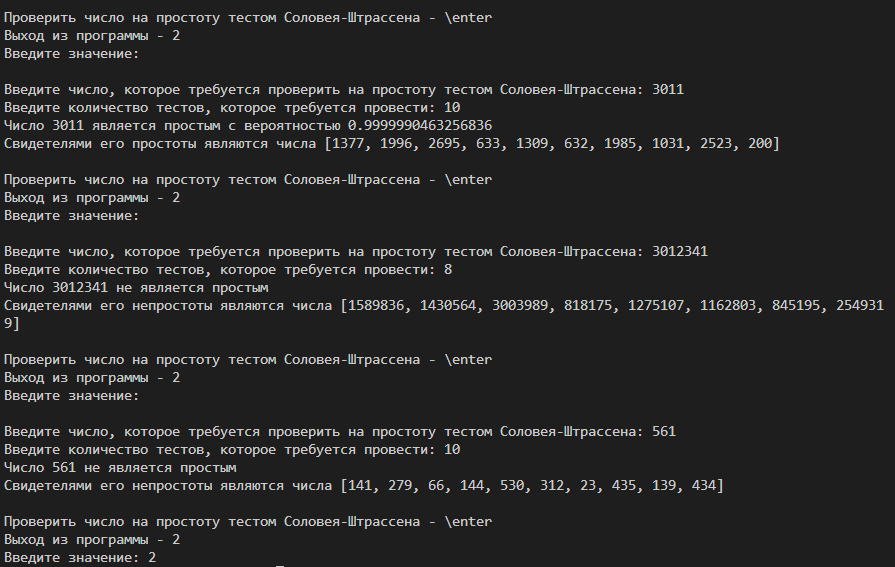
\includegraphics[width=0.8\textwidth]{pic1.png}
    \caption{}
\end{figure}

\setminted[python]{linenos,breaklines=true, fontsize=\small, style=bw}
    \subsection{Код программы, реализующей рассмотренный алгоритм}
        \inputminted{python}{lab6.py}

\end{document}